\documentclass[t,usepdftitle=false]{beamer}

\usepackage[utf8]{inputenc}
\usetheme{Singapore}
\usepackage{xcolor}
\setbeamertemplate{footline}[frame number]

\usepackage{etex}
\usepackage{pictex}
\usepackage{tikz}
\usetikzlibrary{shapes,arrows}
\usepackage{pgfplots}

\usepackage{amsmath}

% \setbeamercovered{transparent}
%\usecolortheme{crane}
\title[Simulation]{Discrete event simulation}

\author[Fabian Bastin]{Fabian Bastin \\ \url{fabian.bastin@umontreal.ca} \\ Université de Montréal -- CIRRELT -- IVADO -- Fin-ML}
\date{}

\def\bu{\boldsymbol{u}}
\def\cS{\mathcal{S}}

\begin{document}
\frame{\titlepage}

% ------------------------------------------------------------------------------------------------------------------------------------------------------
\begin{frame}
	\frametitle{Basic concepts}
	
	\begin{description}
		\item[System]
		collection d'entités qui agissent et interagissent afin d'accomplir une certaine fin logique.\\
		L'état d'un système est la collection de variables nécessaires pour décrire un système à un instant particulier.
		\item[Model]
		description simplifiée d'un système, dans le but d'évaluer sa performance ou l'effet de certaines décisions.
		\item[Simulation]
		faire évoluer le modèle d'un système en fournissant les entrées appropriées, puis observer et analyser les résultats.
	\end{description}
	
	\mbox{}
	
	Two main system types: discrete and continuous.Deux types principaux de systèmes: discrets et continus.
	
\end{frame}

\begin{frame}
	\frametitle{Models}
	
	Physical vs mathematical model.
	
	\mbox{}
	
	Analytical model, numerical model, model with simulation.

\mbox{}

Reference textbook: 
A. M. Law, Simulation Modeling and Analysis, fifth edition, McGraw-Hill, USA, 2015.

\end{frame}

\begin{frame}
\frametitle{Event approach}

Hypothèse: système dans lequel les variables d'état ne peuvent changer qu'en un nombre dénombrable de points dans le temps.

\mbox{}

Suite d'événements $e_0, e_1, e_2\ldots$, survenant aux instants $0 \leq t_0 \leq t_1 \leq t_2 \leq \ldots$. 

\mbox{}

${\cS_i}$: état du système immédiatement après ${e_i}$.

\mbox{}

temps de la simulation: valeur courante de ${t_i}$.

\mbox{}

$(t_i,\cS_i)$ doit contenir assez d'information pour poursuivre la simulation (sauf les valeurs des variables aléatoires générées lors des événements $e_j$ pour $j > i$).

\end{frame}

\begin{frame}
\frametitle{Discrete events}

\begin{center}
%%  Evolution of a general discrete-event model.
\hspace{0.5cm}
\beginpicture
\setcoordinatesystem units <7pt,7pt>
%%  72.27pt = 1in
\setplotarea x from 0 to 36, y from 0 to 10
\axis left
  label {\lines {\emph{state}\cr\vbox to 95pt{\hbox to 1.5pt{\null }} \cr}
         \hskip 9pt } /

\axis bottom
  label {\hbox to 4.0in {\hfill \emph{time}}}
  ticks length <4pt> withvalues 
     0 $t_1$ $t_2$ $t_3$ $t_4$ $t_5$ $t_6$ /
  at 0.0 6.0 7.5 12.5 18.0 25.2 30.0 / /

\axis bottom /
\put {$\rightarrow$} at 36.0 -0.1 
\put {$\uparrow$}    at 0.0 10.0 
\multiput {$\bullet$} at
  0.0 2.0
  6.0 1.6
  7.5 2.7
 12.5 6.1
 18.0 5.1
 25.2 2.6
 30.0 4.0 /
\putrule from  0.0 2.0 to  6.0 2.0
\putrule from  6.0 1.6 to  7.5 1.6
\putrule from  7.5 2.7 to 12.5 2.7
\putrule from 12.5 6.1 to 18.0 6.1
\putrule from 18.0 5.1 to 25.2 5.1
\putrule from 25.2 2.6 to 30.0 2.6
\putrule from 30.0 4.0 to 32.0 4.0 
\endpicture
\end{center}

\end{frame}

\begin{frame}
\frametitle{General framework}

\begin{itemize}
\item
Programme principal.
\item
Horloge de simulation.
\item
Liste d'événements.
\item
Routines de génération de nombres aléatoires.
\item
Compteurs statistiques.
\item
Génération de rapport.
\end{itemize}

Evénement: action, schedule, cancel.

\end{frame}

\begin{frame}

\tikzstyle{decision} = [diamond, draw, fill=blue!20,
    text width=2.5cm, text badly centered, node distance=1cm, inner sep=0pt]
\tikzstyle{block} = [rectangle, draw, fill=blue!20,
    text width=2.5cm, text centered, rounded corners, minimum height=4em]
\tikzstyle{line} = [draw, very thick, color=black!50, -latex']
\tikzstyle{cloud} = [draw, ellipse,fill=yellow!20, node distance=1cm,
    minimum height=2em]

\begin{footnotesize}
\begin{center}
\begin{tikzpicture}[scale=0.1, node distance = 1cm, auto]
    % Place nodes
    \node [block] (init) {Initialisation};
    \node [text width=2.2cm, cloud, left of=init, node distance=4.0cm] (clock) {Horloge de simulation mise à 0};
    \node [text width=2.5cm, cloud, right of=init, node distance=4.0cm] (system) {Planification du ou des premiers(s) événement(s)};
    \node [text width=2.1cm, cloud, below of=init, node distance=3.0cm] (premier) {Dépilement du premier événement};
    \node [text width=2.1cm, block, below of=premier, node distance=3.0cm] (event) {Gestion de l'événement actuel};
    \node [text width=2.1cm, block, below of=event, node distance=3.0cm] (schedule) {Planification du ou des événements en découlant.};
    \node [block, left of=schedule, node distance=5.0cm] (update) {Dépilement du prochain événement et avancement de l'horloge de simulation};
    \node [text width=2.1cm, decision, below of=schedule, node distance=4.0cm] (decide) {Liste d'événements vide ou événement de fin?};
    \node [block, below of=decide, node distance=4.5cm] (stop) {Arrêt};
    % Draw edges
    \path [line] (init) -- (premier);
    \path [line] (premier) -- (event);
    \path [line] (event) -- (schedule);
    \path [line] (schedule) -- (decide);
    \path [line] (decide) -| node [near start, color=black] {non} (update);
    \path [line] (update) |- (event);
    \path [line] (decide) -- node [, color=black] {oui}(stop);
    \path [line,dashed] (clock) -- (init);
    \path [line,dashed] (system) -- (init);
\end{tikzpicture}
\end{center}
\end{footnotesize}

\end{frame}

\begin{frame}

\tikzstyle{decision} = [diamond, draw, fill=blue!20,
    text width=2.5cm, text badly centered, node distance=2.5cm, inner sep=0pt]
\tikzstyle{block} = [rectangle, draw, fill=blue!20,
    text width=2.5cm, text centered, rounded corners, minimum height=4em]
\tikzstyle{line} = [draw, very thick, color=black!50, -latex']
\tikzstyle{cloud} = [draw, ellipse,fill=yellow!20, node distance=2.5cm,
    minimum height=2em]

\begin{footnotesize}
\begin{center}
\begin{tikzpicture}[scale=0.1, node distance = 1cm, auto]
    % Place nodes
    \node [text width=3cm, block, below of=premier, node distance=2cm] (event) {Gestion événement actuel};
    \node [text width=3cm, block, below of=event, node distance=2cm] (schedule) {Planification des événements en découlant.};
    \node [block, left of=schedule, node distance=4.5cm] (update) {Dépilement événement et avancement horloge};
    \node [text width=2.cm, decision, below of=schedule, node distance=2.5cm] (decide) {Liste d'év. vide ou év. de fin?};
    \node [block, below of=decide, node distance=2.5cm] (stop) {Arrêt. Impression rapport.};
    % Draw edges
    \path [line] (event) -- (schedule);
    \path [line] (schedule) -- (decide);
    \path [line] (decide) -| node [near start, color=black] {non} (update);
    \path [line] (update) |- (event);
    \path [line] (decide) -- node [, color=black] {oui}(stop);
\end{tikzpicture}
\end{center}
\end{footnotesize}

\end{frame}

\begin{frame}
\frametitle{Queueing systems}

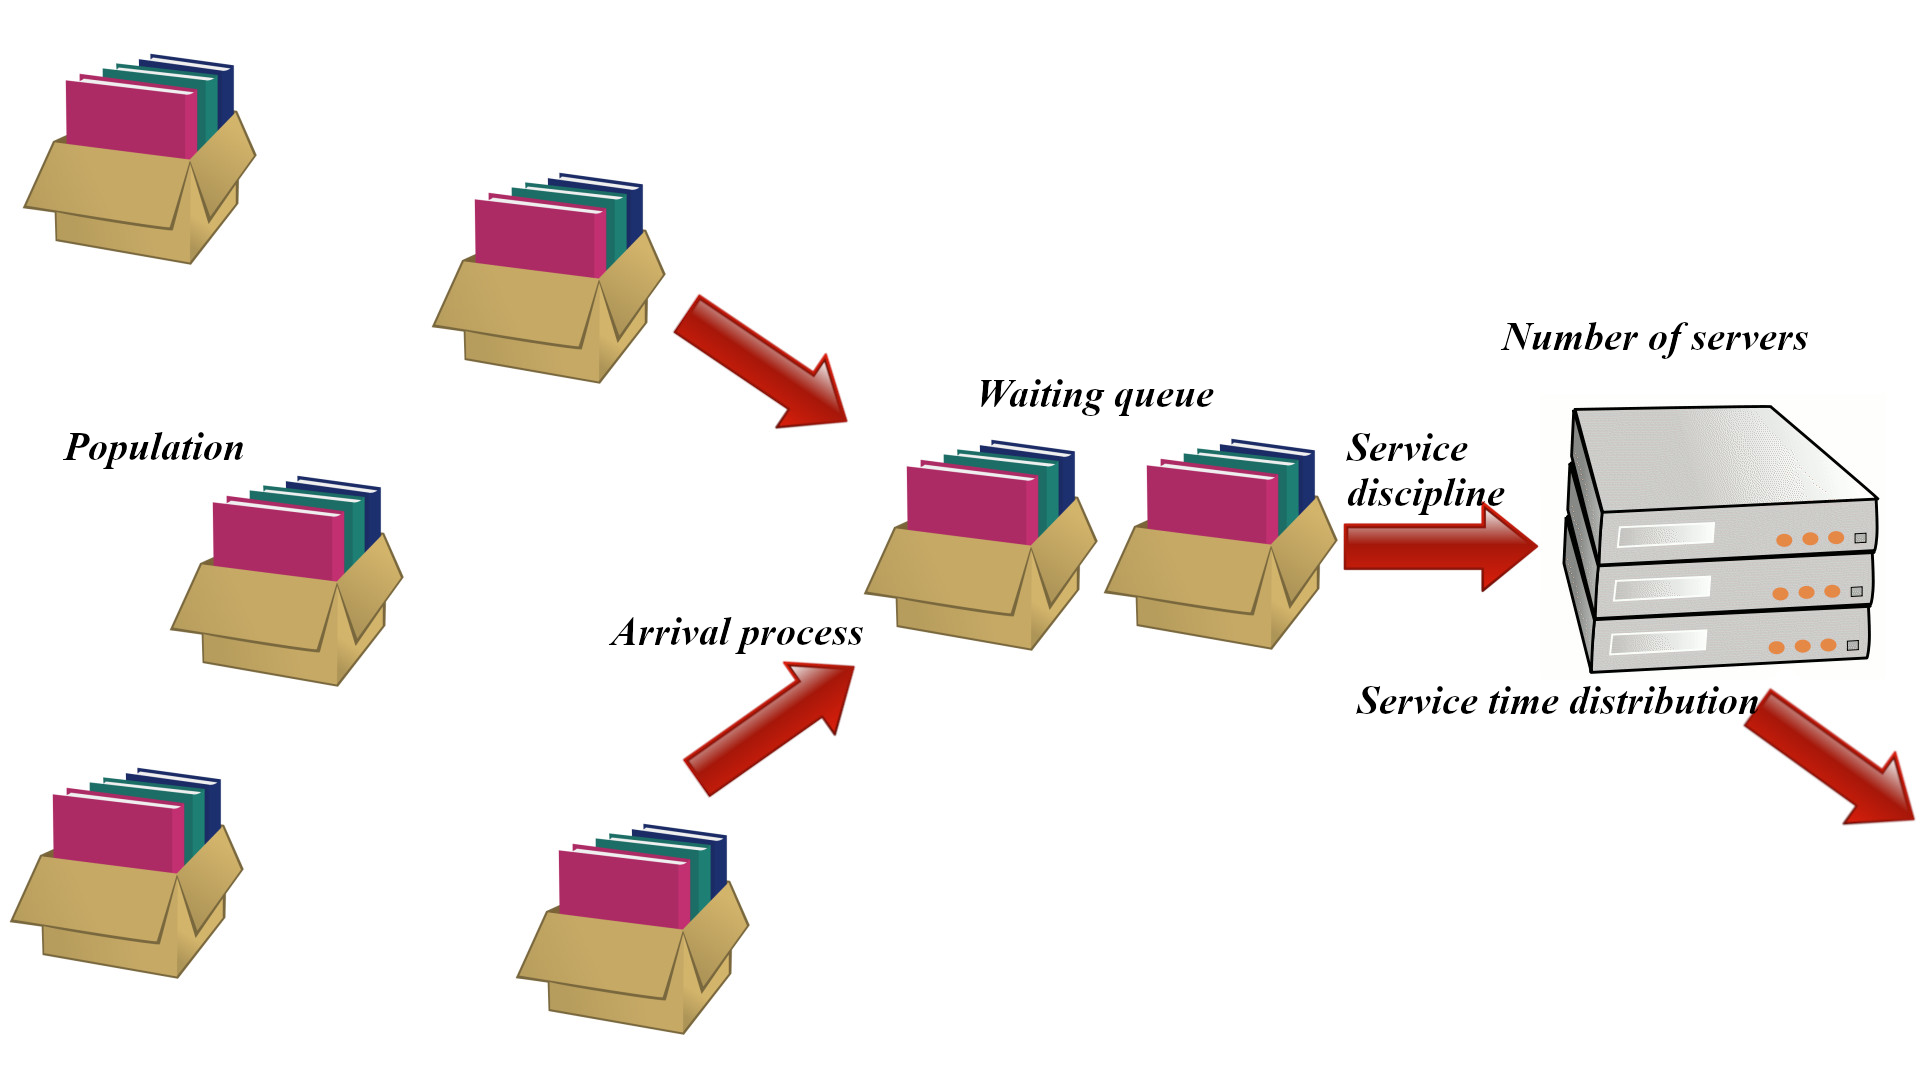
\includegraphics[width=\textwidth]{imgs/queue-labels.png}

\end{frame}

\begin{frame}
\frametitle{Kendall notation}

$$
A/S/c/K/N/SD
$$

\mbox{}

\begin{description}
	\item[$A$]
Arrival process
	\item[$S$]
Service time distribution
	\item[$c$]
Number of servers
	\item[$K$]
Waiting list maximum length
	\item[$N$]
Population size
	\item[$SD$]
Service discipline
\end{description}
 
\end{frame}

\begin{frame}
\frametitle{Notation}

\begin{description}
	\item[$G$]
	General
	\item[$I$]
	Independent
	\item[$M$]
	Markovian or memoryless
\end{description}

\mbox{}

Defaults:
\begin{itemize}
	\item
	Infinite buffer capacity
	\item
	Infinite population size
	\item
	FCFS (First-Come-First-Served) service discipline
\end{itemize}

\mbox{}

Memoryless property:
$$
P[X > x +a \,|\, X > a] = P[X > x]
$$
Continuous: exponential distribution\\
Discrete: geometric distribution 

\end{frame}

\begin{frame}
\frametitle{Example: GI/G/1 queue}

$$
G/G/1 = G/G/1/\infty/\infty/FCFS
$$

We also write $GI/G/1$ to stress that the service times are independent.

\mbox{}

The clients arrive one by one, one being served at a time, under a FCFS priority, with
\begin{itemize}
\item
${S_i}$: service time of client $i$, with cdf $G$;
\item
${A_i}$: inter-arrival time between clients $i$ and $i+1$, with cdf $F$.
\end{itemize}
We assume $S_i$ and $A_i$ mutually independent.

\end{frame}

\begin{frame}
\frametitle{Example: GI/G/1 queue}

The first client arrives at time ${A_0}$ in an empty system.

\mbox{}

Nous souhaitons simuler ce système pour une durée ${T}$ et calculer
l'attente moyenne par client et la longueur moyenne de la file d'attente.
Les types d'événements sont
\begin{enumerate}
\item
arrivée;
\item
départ;
\item
fin de la simulation.
\end{enumerate}
Les variables aléatoires (indépendentes) à générer sont $A_1, A_2,
A_3, \dots$ et $S_1, S_2, S_3, \dots$.

\end{frame}

\begin{frame}
\frametitle{Example: GI/G/1 queue}

\begin{itemize}
\item
${W_i}$, le temps d'attente du client $i$;
\item
${Q(t)}$, la longueur de la file d'attente au temps $t$;
\item
${N_c(t)}$, le nombre de clients ayant débuté leur service durant l'intervalle $[0,t]$.
\end{itemize}
Supposons que nous voulons calculer, pour l'intervalle $[0,T]$,
l'\emph{attente moyenne} par client,
\[
 {\overline{W}_{N_c(T)}} = {1\over N_c(T)} \sum_{i=1}^{N_c(T)} W_i;
\]
et la \emph{longueur moyenne} de la file d'attente:
\[
 {\overline{Q}_T} = {1\over T} \int_0^T Q(t) dt.
\]

\end{frame}

\begin{frame}
\frametitle{Example: GI/G/1 queue}

Cette dernière intégrale est facile à calculer par simulation.

\mbox{}

Pour chaque \emph{client}, nous créons un \emph{objet} contenant l'instant  d'arrivée et la durée de service.

\mbox{}

Variables d'état: liste des clients en attente et la liste les clients en service.

\mbox{}

+ horloge de simulation,
compteurs statistiques (au besoin), \emph{liste} des événements futurs prévus, 
 par ordre chronologique, et une procédure pour chaque type d'événement.
 
\end{frame}

\begin{frame}
\frametitle{Queueing system simulation}

\begin{small}
\begin{description}
\item[Arrivée]
Générer $A$ selon $F$ et prévoir une autre arrivée 
    dans $A$ unités de temps;\\
Créer le nouveau client et noter son instant d'arrivée;\\
Générer sa durée de service $S$ selon $G$;\\
{\bf Si} (serveur est occupé) {\bf alors}\\
\quad Insérer ce client dans la liste des clients en attente;\\
{\bf sinon}\\
\quad   Insérer le client dans la liste des clients en service;\\
\quad   Prévoir son départ dans $S$ unités de temps; \\
Mise à jour des statistiques voulues.
\item[Départ]
Enlever le client de la liste des clients en service;\\
{\bf Si} la file d'attente n'est pas vide {\bf alors}\\
\quad  Enlever le premier client de la liste d'attente;\\
\quad  L'insérer dans la liste des clients en service;\\
\quad  Récupérer son $S$ et prévoir son départ dans 
       $S$ unités de temps;\\
Mise à jour des statistiques voulues.
\item[Fin-de-la-Simulation]
Imprimer un rapport et terminer le programme.
\end{description}
\end{small}
\end{frame}

\begin{frame}
\frametitle{Simulation}

Démarrer la simulation:
\begin{itemize}
\item
initialiser des variables et compteurs,
\item
prévoir la ``Fin-de-la-Simulation'' au temps $T$
\item
générer $A$ selon $F$ et prévoir la première ``Arrivée'' dans $A$ unités de temps,
\item
lancement de la simulation.
\end{itemize}

\mbox{}

L'exécution de la simulation consiste simplement à répéter la boucle
suivante:\\
{\bf Répéter:} exécuter le prochain événement
     dans la liste d'événements\\
{\bf jusqu'à:} la liste des événements prévus est vide,\\
\quad    ou bien un événement stoppe la simulation.

\end{frame}

\begin{frame}
\frametitle{Simulation sans liste d'événements.}

Pas toujours indispensable de recourir à l'approche par événements.

\mbox{}

Exemple: récurrence de Lindley:
\[
 W_1 = 0,\quad W_{i+1} = \max(0,\; W_i + S_i - A_{i+1}).
\]

Nous pouvons ainsi facilement simuler pour un nombre fixe de clients (au lieu d'un horizon de temps $T$ fixe).

\mbox{}

Le formulation du programme basée sur la récurrence de Lindsley revient à traiter un problème d'intégration sur $[0,1)^t$.

\end{frame}

\begin{frame}
\frametitle{Récurrence de Lindley}

Supposons que nous souhaitions estimer $E[\overline{W}_{100}]$ par
${\overline{W}_{100}}$:
\[
{\overline{W}_{100}} = \frac{1}{100} \sum_{i=1}^{100} W_i.
\]

\mbox{}

Il nous faut $A_1, S_1, A_2, S_2, \dots, A_{99}, S_{99}$.
Si on pose ${A_i} = F^{-1}(U_{2i-1})$ et ${S_i} = G^{-1}(U_{2i})$, où
$U_j$, $j = 1,\ldots,99$, sont des variables aléatoires uniformes sur
$(0,1)$, alors $\overline{W}_{100} = f(U_1,\dots,U_{198})$ ($f$ étant de
forme inconnue dans le cas présent).

\mbox{}

Nous avons donc $t=198$, i.e., 
\[
  E[\overline{W}_{100}] = \int_{[0,1)^{198}} f(\bu)d\bu.
\]

\end{frame}

\begin{frame}
\frametitle{Nombre aléatoire de clients}

Par contre, si nous voulons simuler $\overline{W}_{N_c(T)}$, le nombre de clients
$N_c(T)$ est aléatoire et non borné.
Nous devrions donc choisir $t=\infty$ comme dimension.

\end{frame}

\begin{frame}
\frametitle{Approche par processus}

Un processus est une séquence temporellement ordonnée d'événements interreliés, séparés par certains intervalles de temps,
qui décrit l'expérience entière d'une ``entité'' comme celle-ci évolue à travers un ``système''.
Un système ou un modèle de simulation peut avoir différents types de
processus.

\mbox{}

Une routine sera associée à chaque processus du modèle, décrivant son
histoire entière à travers le système.

\mbox{}

Au contraire de l'approche par événements, une routine de processus
contient explicitement le passage du temps simulé et a généralement de
multiples points d'entrée.

\end{frame}

\begin{frame}
\frametitle{Processes vs Events}

Une simulation utilisant l'approche par processus évolue aussi au
cours du temps en exécutant les événements dans l'ordre de leur
occurence.

\mbox{}

En interne, les approches par événement et par processus sont donc
très similaires.

\mbox{}

Pour l'utilisateur, le raisonnement soit
différent, et puisse parfois (mais pas toujours) être plus naturel pour l'approche par processus.

%\mbox{}

%En outre, l'approche par processus est souvent plus lente en terme de
%temps d'exécution, puisque le simulateur doit au final traiter des
%événements, et gérer des processus pouvant être concurrents.

\end{frame}

\end{document}
